\ifdefined\SHOWCASE
  \documentclass[10pt,twocolumn]{article}
\else
  \documentclass[12pt]{article}
\fi

\usepackage{fontspec}
\setmainfont{Times New Roman}[
  Path=/System/Library/Fonts/Supplemental/,
  UprightFont=Times New Roman.ttf,
  BoldFont=Times New Roman Bold.ttf,
  ItalicFont=Times New Roman Italic.ttf,
  BoldItalicFont=Times New Roman Bold Italic.ttf
]
\usepackage{geometry}
\ifdefined\SHOWCASE
  \geometry{margin=0.68in,columnsep=0.24in}
\else
  \geometry{margin=1.25in}
\fi
\usepackage{microtype}
\usepackage{setspace}
\ifdefined\SHOWCASE
  \setstretch{1.04}
\else
  \doublespacing
\fi
\usepackage{amsmath,amssymb,mathtools,bm}
\usepackage{booktabs,threeparttable,tabularx,array,makecell}
\usepackage{graphicx}
\usepackage{caption}
\usepackage{subcaption}
\usepackage{enumitem}
\usepackage{footmisc}
\usepackage{csquotes}
\usepackage{xspace}
\usepackage{xcolor}
\usepackage{xurl}
\ifdefined\SHOWCASE
  \usepackage{titlesec}
\fi
\usepackage[hidelinks]{hyperref}
\usepackage[capitalize,noabbrev]{cleveref}
\ifdefined\SHOWCASE
  \usepackage[
    backend=biber,
    bibstyle=apa,
    citestyle=numeric-comp,
    sorting=none,
    giveninits=true,
    maxbibnames=99,
    doi=true,
    url=true,
    isbn=false
  ]{biblatex}
\else
  \usepackage[
    backend=biber,
    style=apa,
    sorting=nyt,
    giveninits=true,
    maxcitenames=2,
    maxbibnames=99,
    uniquename=false,
    doi=true,
    url=true,
    isbn=false
  ]{biblatex}
\fi
\addbibresource{references.bib}
\DeclareLanguageMapping{english}{english-apa}
\urlstyle{same}
\Urlmuskip=0mu\relax
\DeclareFieldFormat{doi}{\par\noindent\url{https://doi.org/#1}}
\DeclareFieldFormat{url}{\par\noindent\url{#1}}

\DeclareNameAlias{sortname}{family-given}
\DeclareDelimFormat{multinamedelim}{\addcomma\space}
\DeclareDelimFormat{finalnamedelim}{\addspace and\space}
\ifdefined\SHOWCASE\else
  \DeclareDelimFormat{nameyeardelim}{\addspace}
  \renewcommand*{\nameyeardelim}{\addspace}
\fi
\renewbibmacro*{in:}{%
  \ifentrytype{article}
    {}
    {\printtext{\bibstring{in}\intitlepunct}}}
\setlength{\bibitemsep}{0.45\baselineskip}
\ifdefined\SHOWCASE
  \defbibenvironment{bibliography}
    {\list
      {\printtext[labelnumberwidth]{\mkbibbrackets{\printfield{labelnumber}}}}
      {\setlength{\labelwidth}{\labelnumberwidth}%
       \setlength{\leftmargin}{\labelwidth}%
       \setlength{\labelsep}{\biblabelsep}%
       \addtolength{\leftmargin}{\labelsep}%
       \setlength{\itemsep}{\bibitemsep}%
       \setlength{\parsep}{\bibparsep}}}
    {\endlist}
    {\item}
\fi

\captionsetup{
  font=small,
  labelfont=bf,
  justification=raggedright,
  singlelinecheck=false
}
\captionsetup[table]{position=top}
\captionsetup[figure]{position=bottom}

\ifdefined\SHOWCASE
  \titleformat{\section}[block]
    {\normalfont\large\bfseries\raggedright}
    {\thesection}{0.55em}{}
  \titlespacing{\section}{0pt}{1.55ex plus 0.35ex minus 0.15ex}{0.7ex}
  \titleformat{\subsection}[block]
    {\normalfont\normalsize\bfseries\raggedright}
    {\thesubsection}{0.5em}{}
  \titlespacing{\subsection}{0pt}{1.15ex plus 0.25ex minus 0.1ex}{0.45ex}
  \setlength{\parindent}{1.15em}
  \setlength{\parskip}{0pt}
  \renewcommand{\thefootnote}{[\arabic{footnote}]}
\fi

\newcommand{\E}{\mathbb{E}}
\newcommand{\Var}{\operatorname{Var}}
\newcommand{\Prob}{\mathbb{P}}
\newcommand{\TV}{\operatorname{TV}}
\newcommand{\OMAE}{\operatorname{OMAE}}
\newcommand{\RMSE}{\operatorname{RMSE}}
\newcommand{\LLM}{LLM\xspace}
\newcommand{\HGB}{HGB\xspace}
\newcommand{\CGSS}{CGSS\xspace}
\newcolumntype{Y}{>{\raggedright\arraybackslash}X}

\title{\textbf{Synthetic Respondents without Ambivalence?}\\
A Population-Fidelity Audit of Large Language Model Survey Simulations}
\ifdefined\SHOWCASE
  \author{\ShowcaseAuthor\\\ShowcaseAffiliation}
\else
  \author{}
\fi
\date{}

\begin{document}
\maketitle
\ifdefined\SHOWCASE\else
  \thispagestyle{plain}
\fi

\begin{abstract}
Large language models can generate plausible survey answers without reproducing the population those answers are meant to represent. This article develops an estimand-indexed population-fidelity audit that separates marginal calibration, response heterogeneity, relational structure, and predictive benchmarking. A Monte Carlo study shows why the separation matters: generators with nearly identical univariate fit can produce radically different covariance structures. The audit is then applied to five repeated Qwen3-8B responses for each of 300 profiles sampled from three Chinese General Social Survey waves. The model shifts several item means, cuts response variance by more than half, and raises the housework item's mean absolute correlation with the other attitudes from .049--.078 among weighted human respondents to .437--.507. Across all three waves, every audited property falls outside a reference envelope generated by repeated human samples of the same size. Outcome-informed references remain imperfect for individuals, but a simple joint-donor model recovers both marginal and relational structure far better. Sparse profile information is therefore a real prediction limit, but it is not a sufficient explanation for the recorded language model's population distortion.
\end{abstract}

\noindent\textbf{Keywords:} synthetic respondents; large language models; survey simulation; population fidelity; machine learning; gender attitudes

\section{Introduction}

Large language models can produce answers that sound like survey responses from recognizable social
types. Given a profile describing an older rural man with little education, a model can select a
plausible position on a gender-role question; given a younger urban woman with a university
education, it can generate a different one. This capacity has encouraged proposals to use language
models as experimental subjects, pilot respondents, or even substitutes for expensive human samples
\parencite{argyle2023one,aher2023simulate,dillion2023replace}. The methodological difficulty is that
plausibility is an individual-level judgment, whereas survey inference concerns populations.
Researchers need distributions, disagreement, covariance, subgroup contrasts, and uncertainty---not
merely fluent impersonations.\footnote{The term \emph{synthetic respondent} here refers to an LLM
prompted to answer as a persona. It should not be confused with conventional statistical synthetic
data, which are generated from an explicitly estimated model of observed confidential data.}

Existing audits establish that this distinction can fail in practice. Demographic conditioning can
recover some subgroup patterns, the result described as ``algorithmic fidelity'' by
\textcite{argyle2023one}. Yet language-model samples can also misrepresent opinion distributions,
compress variance, change regression coefficients, react to small prompt changes, and drift when a
proprietary model is updated \parencite{santurkar2023opinions,bisbee2024synthetic,qu2024performance}.
These findings have shifted the question from whether an LLM can ever resemble a human sample to
when resemblance is adequate for a stated analytical use.

Two gaps remain. First, evaluations often move directly from individual or marginal accuracy to a
global verdict on ``fidelity.'' That verdict obscures which property failed. A generator can match
means while erasing covariance, or miss many individuals while still recovering a population
distribution. Second, a failed persona prediction has at least two explanations. Demographic
profiles may contain little information about a person's attitude, or the generator may distort the
information that is available. Without an outcome-informed reference trained on the same profile
features, it is difficult to determine whether sparse profiles are a sufficient explanation for
the observed error.

This article critically assesses persona-based survey simulation and offers a usable correction: a
four-stage \emph{population-fidelity audit}. The audit evaluates (1) marginal calibration,
(2) response heterogeneity, (3) relational structure, and (4) performance relative to transparent
outcome-informed references. The stages are not a new estimator and do not establish a universal
score. They are a decision procedure: researchers specify the downstream estimand, test every
population property that estimand requires, and compare the synthetic error with a reference
distribution obtained from equally sized human samples. A mean-estimation task may require marginal
calibration; a regression, scale, or latent-class analysis additionally requires covariance and
subgroup structure. The emphasis on a staged,
reproducible workflow follows a broader computational-methods tradition in sociology
\parencite{nelson2020computational}.

The evidence has two parts. A Monte Carlo study calibrated to real survey marginals compares a
row-bootstrap generator, an independent-marginals generator, and a deliberately coherent
single-factor generator. All three achieve almost identical mean and distributional fit, but only
the row bootstrap preserves the human correlation matrix. The simulation demonstrates the failure
regime for mean-only validation rather than assuming it.

The real-data illustration uses 31,856 respondents from the 2012, 2018, and 2021 Chinese General
Social Survey (\CGSS) and 300 matched profiles sent to a locally deployed Qwen3-8B model. Five
gender-attitude items create a demanding benchmark because human respondents combine public-sphere
and household beliefs in ways that are not strongly unidimensional. The model is compared with the
matched human answers, weighted population distributions, a marginal prior, multinomial logit,
histogram gradient boosting, and a stratified joint-donor generator. These references receive no
more profile features than the LLM at prediction time, although unlike the zero-shot LLM they learn
from survey outcomes during training.\footnote{The supervised comparison is intentionally asymmetric in training information.
It is not a contest over equal training budgets. Its purpose is to determine whether sparse profile
features impose the particular errors produced by the zero-shot generator.}

The results are substantial and internally consistent for this case. Qwen3-8B's ordinal mean
absolute error is 1.379 on the
five-point scale, compared with 0.923 for histogram gradient boosting. Its average total variation
distance is 0.538 rather than 0.071, and its variance ratio is 0.466 rather than 0.987. More
consequentially, equal-housework attitudes have mean absolute correlations of .437--.507 with the
other items, compared with .049--.078 in the weighted human data. All 15 wave-by-property audit
results fall outside the 95 percent reference envelopes from repeated human samples. The model
therefore creates not only a miscentered population, but a more homogeneous and ideologically
coherent one.

The contribution is methodological and bounded. The article does not claim that all LLMs fail, that
survey-trained prediction models explain human psychology, or that one Chinese gender battery
represents all public opinion. It shows that validation must be indexed to population properties and
that outcome-informed references can test whether limited profile information is a sufficient
explanation for observed distortion. The design does not isolate model architecture from the
absence of task-specific calibration. The accompanying code reproduces the simulation, figures, and
empirical comparisons.

\section{Synthetic Respondents as a Measurement Procedure}

\subsection{The target is a distribution, not a persona}

Let $\bm X_i$ denote the observed profile of respondent $i$, $q_j$ a survey item, and
$Y_{ij}\in\{1,\ldots,K\}$ the human response. A persona-prompted language model produces
\begin{equation}
  \widetilde{Y}^{L}_{ij}
  =
  g_{\theta}\!\left(\bm X_i,q_j,p,s\right),
  \label{eq:generator}
\end{equation}
where $\theta$ denotes the fixed model, $p$ the prompt, and $s$ the decoding seed. A fluent value of
$\widetilde{Y}^{L}_{ij}$ can be plausible conditional on $\bm X_i$ without reproducing the human
conditional distribution
\begin{equation}
  \pi_{ijk}
  =
  \Prob(Y_{ij}=k\mid\bm X_i),
  \qquad k=1,\ldots,K.
  \label{eq:target}
\end{equation}
The gap between \cref{eq:generator} and \cref{eq:target} is the central validation problem.
Pretraining does not directly optimize $g_{\theta}$ for the target survey, population, language,
year, response scale, or estimand. Prompting supplies context but not empirical base rates.

This formulation treats persona simulation as a measurement procedure. The generated response is an
instrument reading produced by a model, prompt, and decoder. As with any instrument, validity is
use-specific. Exact agreement with one respondent is demanding because survey answers contain
idiosyncratic and transient variation. But low individual accuracy does not license arbitrary
aggregate error. A model used to estimate a mean must recover the relevant marginal distribution; a
model used for association or measurement analysis must also recover the joint distribution.

The distinction is increasingly important as LLMs enter social-science workflows
\parencite{demszky2023psychology,chae2025classification}. Classification research can validate
predictions against labels, but synthetic respondents are often invoked precisely where labels are
scarce or absent. That makes explicit external benchmarks more important, not less. Otherwise,
coherent output can create an illusion of understanding: the system produces a complete population
because the researcher asked for one, not because that population has been measured
\parencite{messeri2024illusions}.

\subsection{Four levels of population fidelity}

\Cref{fig:audit-design} summarizes the proposed audit. Each level corresponds to a different
property of the population distribution and a different class of downstream estimands.

\paragraph{Marginal fidelity.}
The first level asks whether the generator recovers category shares, means, and other univariate
features. These quantities are sufficient for a narrow descriptive estimand, but they say little
about relationships among variables. For item $j$, total variation distance is
\begin{equation}
  \TV_j
  =
  \frac{1}{2}\sum_{k=1}^{K}
  \left|\widehat{\pi}^{\,L}_{jk}-\widehat{\pi}^{\,H}_{jk}\right|,
  \label{eq:tv}
\end{equation}
where $L$ and $H$ denote language-model and human distributions.

\paragraph{Heterogeneity fidelity.}
The second level asks whether disagreement is preserved. The variance ratio
\begin{equation}
  R^{V}_{j}
  =
  \frac{\Var(\widetilde{Y}^{L}_{j})}{\Var(Y^{H}_{j})}
  \label{eq:variance}
\end{equation}
equals one under variance recovery. Values below one indicate compression. A model may match a mean
by placing nearly everyone near it, producing misleading standard errors, subgroup overlap, and
latent-class prevalence.

\paragraph{Relational fidelity.}
The third level concerns the joint distribution. This article uses the root mean squared difference
between item-correlation matrices,
\begin{equation}
  \RMSE_R
  =
  \left[
    J^{-2}
    \sum_{j=1}^{J}\sum_{\ell=1}^{J}
    \left(\widehat r^{\,L}_{j\ell}-\widehat r^{\,H}_{j\ell}\right)^2
  \right]^{1/2},
  \label{eq:corr-rmse}
\end{equation}
and errors in demographic regression coefficients. Correlations are not privileged as causal or
latent parameters; they are transparent diagnostics for whether synthetic data preserve
relationships routinely used in social-science analysis.

\begin{samepage}
\paragraph{Predictive benchmarking.}
The fourth level asks whether the generator adds value relative to explicit references. Let
$p_{mij}(k)$ be the probability assigned by model $m$ and
$\widehat\mu_{mij}=\sum_k k p_{mij}(k)$. Ordinal mean absolute error is
\begin{equation}
  \OMAE_m
  =
  \frac{1}{NJ}
  \sum_{i=1}^{N}\sum_{j=1}^{J}
  \left|\widehat\mu_{mij}-Y_{ij}\right|.
  \label{eq:omae}
\end{equation}
\end{samepage}
For the LLM, the primary analysis uses $R=5$ repeated draws,
\begin{equation}
  \widehat\mu_{Lij}
  =
  R^{-1}\sum_{r=1}^{R}\widetilde Y^{L}_{ijr},
  \label{eq:llm-mean}
\end{equation}
while a single-draw version remains a sensitivity analysis. References should include a marginal
prior, an interpretable conditional model, a flexible learner, and---when relational fidelity is
required---a generator that produces joint outcomes. This ladder distinguishes base-rate
calibration from personalization, nonlinear prediction, and joint reconstruction.

The deployment rule is therefore conditional rather than universal: a synthetic sample must pass
the stages required for its intended estimand and outperform a simpler reference that has comparable
access to prediction-time information. In the empirical audit, ``pass'' means that the synthetic
error remains inside the central 95 percent reference envelope obtained by repeatedly drawing human
samples with the same profile-sampling design. Failure at a required stage is not repaired by
fluency at the individual level.

\begin{figure*}[!t]
  \centering
  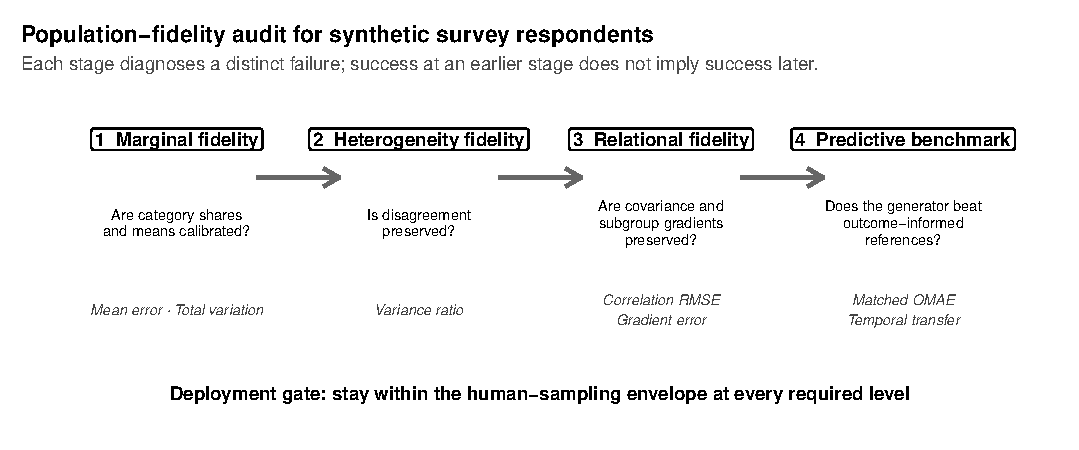
\includegraphics[width=\textwidth]{figures/audit_design.pdf}
  \caption{Population-fidelity audit for synthetic survey respondents. The stages are cumulative
  only relative to an intended estimand: passing marginal calibration does not establish
  heterogeneity or relational fidelity.}
  \label{fig:audit-design}
\end{figure*}

\subsection{Why gender attitudes are a hard structural test}

The empirical illustration uses gender attitudes because meaningful inconsistency is common.
Gender operates across institutional, interactional, and individual settings
\parencite{risman2004gender}. Support for women's education or employment can coexist with
traditional expectations inside marriage. Work on the uneven gender revolution and multiple
egalitarianisms therefore treats ambivalence and domain differentiation as substantive patterns,
not merely noise \parencite{england2010gender,knight2017egalitarianism,scarborough2019attitudes}.

The Chinese case sharpens this test. Public participation by women has long had institutional
legitimacy, while domestic labor remains strongly organized through households. Research using
Chinese surveys accordingly distinguishes work and family spheres and documents variation across
cohorts, regions, gender, and education
\parencite{shu2004education,qian2020separating,yang2023mosaic}. A language model may instead map a
profile to a compressed social type---``traditional'' or ``modern''---and carry that type across
every item. If so, the synthetic data will look more unidimensional than the human data.

This battery is not a definitive measurement model. Four items are traditional statements and one
asks positively about equal housework. The housework item is a single indicator, so weak covariance
can reflect content, wording, acquiescence, or item-specific error.\footnote{The audit therefore
uses the observed weak association as a benchmark property to be reproduced. It does not claim that
one item identifies a complete household-gender latent variable.} This limitation makes the test
more conservative: the LLM is evaluated on whether it reproduces the empirical structure, not on
whether one theoretical explanation for that structure is true.

\section{Audit Design}

\subsection{Reference ladder}

\Cref{tab:reference-ladder} makes the comparison logic explicit. The weighted prior observes outcome
frequencies but ignores profiles. Multinomial logit estimates additive conditional associations.
Histogram gradient boosting (\HGB) permits nonlinearities and interactions
\parencite{mullainathan2017machine,pedregosa2011scikit}. A stratified joint-donor generator samples
complete five-item response vectors from training respondents matched on wave, sex, education
group, and urban residence; it is deliberately simple but preserves respondent-level dependence.
Qwen3-8B observes no task-specific survey outcomes and is evaluated zero-shot. The references are
not psychological theories. They diagnose what can be reconstructed when survey outcomes are
available.

\begin{table*}[!htbp]
\centering
\caption{Reference ladder for diagnosing synthetic-respondent failure}
\label{tab:reference-ladder}
\begin{threeparttable}
\small
\begin{tabularx}{\textwidth}{lYYYY}
\toprule
Method & Outcome information & Profile information & Diagnostic role & Main limitation \\
\midrule
Weighted marginal prior
  & Training-fold category shares
  & None
  & Base-rate calibration without personalization
  & Cannot recover subgroup differences \\
Multinomial logit
  & Training-fold individual outcomes
  & Same features shown to the LLM
  & Transparent conditional benchmark
  & Additive linear predictor on the log-odds scale \\
Histogram gradient boosting
  & Training-fold individual outcomes
  & Same features shown to the LLM
  & Flexible outcome-informed benchmark
  & Task-specific and outcome-informed \\
Stratified joint donor
  & Complete training-fold response vectors
  & Wave, sex, education group, and residence
  & Transparent benchmark for joint reconstruction
  & Coarse matching and task-specific outcomes \\
Qwen3-8B
  & No CGSS outcomes
  & Persona text built from the same features
  & Zero-shot test of implicit base rates and conditioning
  & Model-, prompt-, and decoding-specific \\
\bottomrule
\end{tabularx}
\begin{tablenotes}[flushleft]
\footnotesize
\item Notes: ``Same features'' refers to survey wave, province, sex, age, education, hukou,
urban residence, partnership status, and relative economic position. The comparison equalizes
prediction-time covariates, not training information.
\end{tablenotes}
\end{threeparttable}
\end{table*}

\subsection{Monte Carlo study}

The simulation demonstrates why the first two audit stages cannot establish the third. The target
population is calibrated to the weighted marginal distributions and joint response patterns of
complete cases in \CGSS 2021. Each replication draws $n=300$ observations under three data-generating
procedures:

\begin{enumerate}[leftmargin=2em]
  \item \textbf{Row bootstrap}: sample complete respondent rows with probability proportional to the
  survey weight. This preserves the empirical joint distribution in expectation.
  \item \textbf{Independent marginals}: draw each item independently from its weighted empirical
  category probabilities. Marginal distributions are correct, but covariance is removed.
  \item \textbf{Coherent factor}: draw five latent normal variables with a common-factor correlation
  of .65 and discretize them using the empirical marginal thresholds. Marginals remain correct while
  coherence is deliberately inflated.
\end{enumerate}

The design uses 1,000 replications with a fixed seed. Performance is measured by mean absolute item
error, average item-level total variation, mean variance ratio, correlation-matrix RMSE, and the mean
absolute correlation between the housework item and the first four items.\footnote{For item $j$,
total variation is $\frac{1}{2}\sum_{k=1}^{5}|p_{jk}^{\mathrm{synthetic}}-
p_{jk}^{\mathrm{human}}|$. It ranges from zero for identical category distributions to one for
disjoint distributions.} The row bootstrap is an
empirically calibrated positive control, not a proposed replacement for a survey. The boundary cases are the
independent and coherent generators: both should pass marginal tests while failing for opposite
reasons at the relational stage.

\subsection{Uncertainty and evidentiary status}

The simulation results are finite-sample regularities, not analytical theorems. Monte Carlo standard
errors are reported in the online supplement. Empirical uncertainty comes from 2,000
profile-cluster bootstrap replications within survey wave. A sampled profile carries all five items
and all repeated model draws with it; neither items nor repeats are resampled independently.
Intervals therefore describe uncertainty conditional on the matched 300-profile design and the
fixed full-sample human benchmark. They do not reproduce every stage of the original multistage
survey sample.

A separate calibration exercise repeats the exact stratified, probability-proportional-to-weight
profile draw 1,000 times within each wave, with $n=100$ each time. Every sampled human population is
compared with the full weighted benchmark using the five audit metrics. The central 95 percent range
of those errors is a sampling reference envelope, not a confidence interval for the finite \CGSS
sample. It operationalizes the deployment rule by showing how far an equally sized human sample
would ordinarily depart from the survey benchmark.

\section{Empirical Illustration: Gender Attitudes in China}

\subsection{Human benchmark}

The human benchmark uses \CGSS 2012, 2018, and 2021
\parencite{cgssdata}. \CGSS is a repeated cross-sectional, multistage probability survey of adults in
China. The analysis requires a valid housework response, at least three valid responses among the
other four items, complete profile variables, and a positive survey weight. The resulting samples
contain 11,668 respondents in 2012, 12,478 in 2018, and 7,710 in 2021, totaling 31,856.

The items ask whether respondents agree that (A421) men should focus on careers and women on family,
(A422) men are naturally more capable than women, (A423) marrying well is better for a woman than
doing well, (A424) women should be dismissed first during an economic downturn, and (A425) spouses
should share housework equally. Responses range from 1 (completely disagree) to 5 (completely agree).
A421--A424 are reverse-coded as $6-Y$, while A425 remains unchanged, so every reported score runs
from 1 to 5 with higher values indicating greater egalitarianism.

The full weighted sample establishes the population benchmark for means, category shares, variances,
and Pearson correlations. Unweighted Pearson and polychoric correlations are reported as sensitivity
checks. Survey weights are also used for human regression gradients because the target is the
sampled population rather than an unweighted convenience sample \parencite{solon2015weighting}. The
analyses are descriptive; references to demographic ``effects'' are avoided because the repeated
cross-sections do not identify causal effects.\footnote{Sex, education, age, hukou, and residence
are treated as conditioning variables and social locations, not randomized treatments.}

\subsection{Matched persona sample}

One hundred respondents are selected from each wave. Sampling is stratified by sex, education group,
and urban residence. Stratum allocations follow weighted population shares, and respondents are
selected within strata with probabilities proportional to their survey weights. Each profile
contains survey year, province, sex, age, years of education, hukou, urban residence, partnership
status, and relative household economic position. The model-facing file excludes all five human
answers.\footnote{``Matched'' means that the LLM, human benchmark, and out-of-fold reference
predictions are evaluated on the same 300 respondent records. It does not refer to propensity-score
matching or to pairing different respondents on observed covariates.}

The design therefore supports three comparisons: the synthetic sample against the full weighted
population, synthetic answers against the same respondents' answers, and synthetic subgroup
patterns against those estimated in the full sample. Matching does not turn the observed answer
into a perfectly measured latent attitude. It makes the information set and evaluation target
auditable.

\subsection{LLM generation and prompt ablation}

The audit uses the open-weight Qwen3-8B model \parencite{qwen2025technical}, executed locally through
Ollama 0.31.1 on an Apple M4 computer with 24 GB of unified memory. The exact local model digest is
recorded in the supplement. The model runs in non-thinking mode with temperature .7, top-$p$ .9,
and a recorded seed. The main Chinese prompt asks the model to answer as the described respondent,
gives verbal labels and their unique numerical mapping, and requires a JSON object. Responses are
accepted only when all five keys are present, scores fall between 1 and 5, and verbal labels agree
with numeric values.

The primary joint condition generates five independently seeded response vectors for every one of
the 300 profiles. These draws define an empirical predictive category distribution for each
profile. The first draw is retained as a prespecified sensitivity analysis so that revised estimates
remain comparable with the original pilot. A second full condition uses the same profiles but tells
the model not to choose politically correct or socially expected answers and omits the verbal-label
validation format. Because those two features change together, that contrast remains a prompt
ablation rather than a factorial causal test.

\begin{samepage}
A targeted follow-up separates joint from independent item presentation. Each item is sent through
a fresh API call with the complete persona repeated, no conversation history, and no access to the
other questions or prior answers. Before the full follow-up run, the primary contrast was fixed as
\[
  \Delta_r
  =
  \overline{|r|}_{\mathrm{joint}}
  -
  \overline{|r|}_{\mathrm{independent}},
\]
where each term averages the absolute correlations between A425 and A421--A424. The joint condition
has five repeats, whereas the independent condition has one response per profile and item. The
profile-bootstrap interval therefore captures profile composition but not repeated-decoding
variation in the independent condition; the contrast is an exploratory presentation test rather
than a complete mechanism experiment. An interval for $\Delta_r$ entirely above zero would support
context-induced coherence. If independent presentation remains above the \CGSS benchmark, the two
mechanisms may coexist.
\end{samepage}

\subsection{Survey-trained references}

The prior, multinomial logit, and \HGB models use the same nine profile features. Numeric predictors
are median-imputed and standardized; province and other categorical predictors are one-hot encoded.
Training weights are normalized to mean one. Hyperparameters are fixed before matched-profile
evaluation.

The main comparison uses five-fold stratified out-of-fold prediction for each item. Each person's
outcome is excluded from the model that predicts that person. The 300 LLM profiles are joined to
these predictions by exact wave and row identifiers. A second design trains on 2012 and 2018 and
tests on 2021. This temporal transfer deliberately removes access to the target year's outcomes,
although the reference models still observe historical labels.

The stratified joint-donor benchmark excludes the matched respondent, locates complete training
respondents in the same wave-by-sex-by-education-by-residence cell, and samples five complete
response vectors using survey weights. Its purpose is not optimal prediction. It tests whether a
transparent outcome-informed procedure can preserve dependence that separate item classifiers
cannot generate.

For every generator, the primary population moments are calculated from its predictive category
distribution. The reference models supply probabilities directly; Qwen3-8B supplies a five-draw
empirical distribution. Total Qwen variance is decomposed into variance between profile-specific
means and average stochastic variance within profiles. The original one-draw variance ratio remains
available as a sensitivity result rather than serving as the primary comparison.

\subsection{Relational diagnostics}

Item structure is summarized by correlation-matrix RMSE and by the mean absolute correlation between
A425 and A421--A424. Human targets use survey-weighted Pearson correlations; unweighted Pearson and
polychoric estimates test whether the weak A425 association is a weighting or ordinal-scaling
artifact. Each of the five joint LLM draws produces a separate 100-profile correlation matrix, and
the resulting diagnostics are averaged rather than treating 500 repeated rows as independent.
Subgroup fidelity is assessed with parallel linear regressions for a four-item
public-attitude index and A425. Each outcome is regressed on sex, years of education, age in decades,
and urban residence. Human regressions use survey weights; synthetic regressions use the sampled
profiles with equal weight because weighting already enters profile selection. Coefficient RMSE and
sign agreement summarize recovery. These regressions are diagnostics of conditional structure, not
substantive causal models.

\section{Results}

\subsection{Mean-only validation accepts structurally wrong populations}

Panel A of \cref{tab:core-results} reports the Monte Carlo study. All three generators have mean
absolute item error between .0546 and .0559, average total variation between .0424 and .0435, and a
mean variance ratio near one. On these metrics, the independent and coherent generators are
indistinguishable from the row bootstrap.

The relational audit reverses that conclusion. Correlation-matrix RMSE is .0505 under row
bootstrapping, .274 under independent marginals, and .371 under the coherent-factor generator. The
housework item's mean absolute correlation is .0905 under the row bootstrap, .0457 under independent
sampling, and .525 under the coherent factor. Mean-only validation would accept all three
populations despite opposite and substantively consequential errors in their joint structure.

\begin{table*}[!htbp]
\centering
\caption{Core simulation and matched-profile results}
\label{tab:core-results}
\begin{threeparttable}
\scriptsize
\setlength{\tabcolsep}{3.2pt}
\begin{tabularx}{\textwidth}{Yrrrrr}
\toprule
Generator or model
& \makecell{OMAE /\\mean error}
& \makecell{Total\\variation}
& \makecell{Variance\\ratio}
& \makecell{Correlation\\RMSE}
& \makecell{A425\\mean $|r|$} \\
\midrule
\multicolumn{6}{l}{\textit{Panel A. CGSS-calibrated Monte Carlo, 1,000 replications}} \\
Row bootstrap & .0547 & .0426 & .997 & .0505 & .0905 \\
Independent marginals & .0546 & .0424 & 1.000 & .274 & .0457 \\
Coherent factor & .0559 & .0435 & .999 & .371 & .525 \\
\addlinespace
\multicolumn{6}{l}{\textit{Panel B. Same 300 empirical profiles}} \\
Weighted marginal prior & .975 & .0965 & .992 & --- & --- \\
Multinomial logit & .935 & .0814 & .982 & --- & --- \\
Histogram gradient boosting & .923 & .0712 & .987 & --- & --- \\
Stratified joint donor & .987 & .0699 & .973 & .0851 & .105 \\
Qwen3-8B, neutral prompt & 1.379 & .538 & .466 & .293 & .468 \\
\bottomrule
\end{tabularx}
\begin{tablenotes}[flushleft]
\footnotesize
\item Notes: Panel A's second column is mean absolute item-mean error; Panel B's is individual
ordinal mean absolute error. Panel A metrics are replication means. Correlation entries average the
three wave-specific values. The prior, logit, and gradient-boosting models generate separate item
probabilities, so relational metrics are undefined for them; the donor and Qwen procedures generate
complete response vectors.
\end{tablenotes}
\end{threeparttable}
\end{table*}

Panel D of \cref{fig:structural} visualizes the failure. The three scenarios occupy nearly the same
position on total variation, while their relational error differs by a factor of more than six.
This is the simulation-backed justification for treating relational fidelity as a separate audit
stage.

\subsection{Observed errors exceed ordinary human sampling variation}

\Cref{tab:sampling-envelope} turns the audit from a metric list into a calibrated decision rule.
Across 1,000 repeated human samples per wave, ordinary samples of 100 respondents have average total
variation below .105 at the upper edge of the central 95 percent reference envelope and
correlation-matrix RMSE below .142. Their variance ratios remain between .846 and 1.141. Qwen3-8B is
outside the corresponding envelope for every metric in every wave---15 of 15 comparisons.

\begin{table*}[!htbp]
\centering
\caption{Qwen3-8B relative to equally sized human sampling envelopes}
\label{tab:sampling-envelope}
\begin{threeparttable}
\small
\begin{tabularx}{\textwidth}{Yrrr}
\toprule
Audit metric & Human 95\% reference range & Qwen range & Waves outside \\
\midrule
Absolute item-mean error & [.036, .168] & [.880, 1.021] & 3 / 3 \\
Total variation & [.046, .105] & [.514, .571] & 3 / 3 \\
Variance ratio & [.846, 1.141] & [.441, .592] & 3 / 3 \\
Correlation-matrix RMSE & [.047, .142] & [.279, .298] & 3 / 3 \\
A425 mean absolute correlation & [.034, .235] & [.437, .507] & 3 / 3 \\
\bottomrule
\end{tabularx}
\begin{tablenotes}[flushleft]
\footnotesize
\item Notes: Each wave contributes 1,000 stratified, probability-proportional-to-weight human
samples of $n=100$. The displayed human range runs from the smallest wave-specific 2.5th percentile
to the largest wave-specific 97.5th percentile, making it a conservative union across waves rather
than a confidence interval. Qwen uses five repeated draws per sampled profile.
\end{tablenotes}
\end{threeparttable}
\end{table*}

The comparison does not imply that \CGSS is error-free. It asks a narrower question: whether Qwen's
departure could plausibly be attributed to using only 100 profiles per wave. The answer is no for
all five audited properties.

\subsection{Qwen3-8B misses item-specific opinion}

\Cref{fig:marginal} shows that error is neither small nor a uniform ideological shift. Under the
neutral prompt, Qwen3-8B approximates the family-role item and produces more egalitarian responses
on male ability. It produces substantially more traditional responses on marriage, employment
protection, and equal housework. Averaged across waves against the full weighted \CGSS distributions,
absolute item-mean error is .942 and total variation is .542.

\begin{figure*}[!htbp]
  \centering
  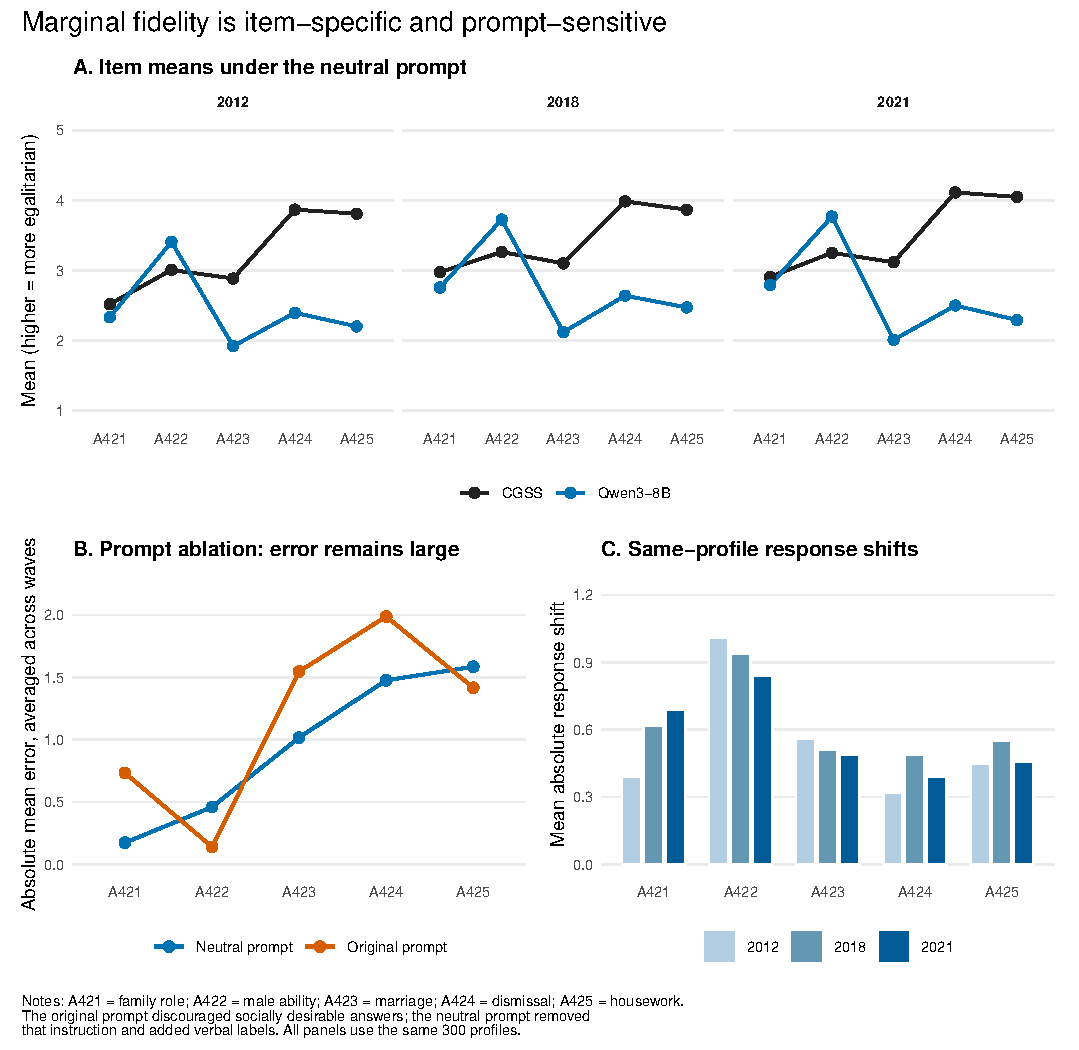
\includegraphics[width=\textwidth]{figures/marginal_fidelity.pdf}
  \caption{Marginal fidelity and prompt ablation. All scores are oriented so that higher values
  indicate greater gender egalitarianism. The original and neutral conditions contain the same 300
  profiles; the ablation changes both the social-desirability instruction and response format.}
  \label{fig:marginal}
\end{figure*}

The largest errors recur across waves. Support for equal housework is understated by 1.61 points in
2012, 1.43 in 2018, and 1.94 in 2021. Opposition to dismissing women first is understated by 1.47,
1.31, and 1.49 points. These differences generate a synthetic population that is much less
supportive of household equality and employment protection than the corresponding survey
populations.

Removing the anti-social-desirability instruction improves but does not repair the distribution.
Mean absolute item error falls from 1.17 under the original prompt to .942 under the neutral prompt;
average total variation falls from .664 to .542. Yet the same-profile mean absolute response shift
is .581 points, demonstrating substantial prompt dependence. Prompt choice changes the severity and
item pattern of error without yielding a condition that passes marginal calibration.

\subsection{The synthetic population is too homogeneous and too coherent}

Panels A and B of \cref{fig:structural} show two distinct structural failures. Across the 15
wave-item cells, the median Qwen-to-human total variance ratio is .412. Within-profile stochastic
variation supplies about 23 percent of Qwen's predictive variance on average, so repeated sampling
adds dispersion without closing the human gap. Compression is most pronounced for marriage and
equal housework in 2012 and 2021. The model is not simply drawing a different population center; it
is suppressing disagreement around that center.

Repeat stability is high but not deterministic. Across waves, 94 percent of A421 profiles and 80
percent of A422 profiles give the same answer in all five draws; the corresponding shares are 69
percent for A423, 58 percent for A424, and 72 percent for A425. The variance decomposition therefore
captures genuine sampling variation, but most of the missing population heterogeneity lies between
profiles rather than within repeated calls.

\begin{figure*}[!htbp]
  \centering
  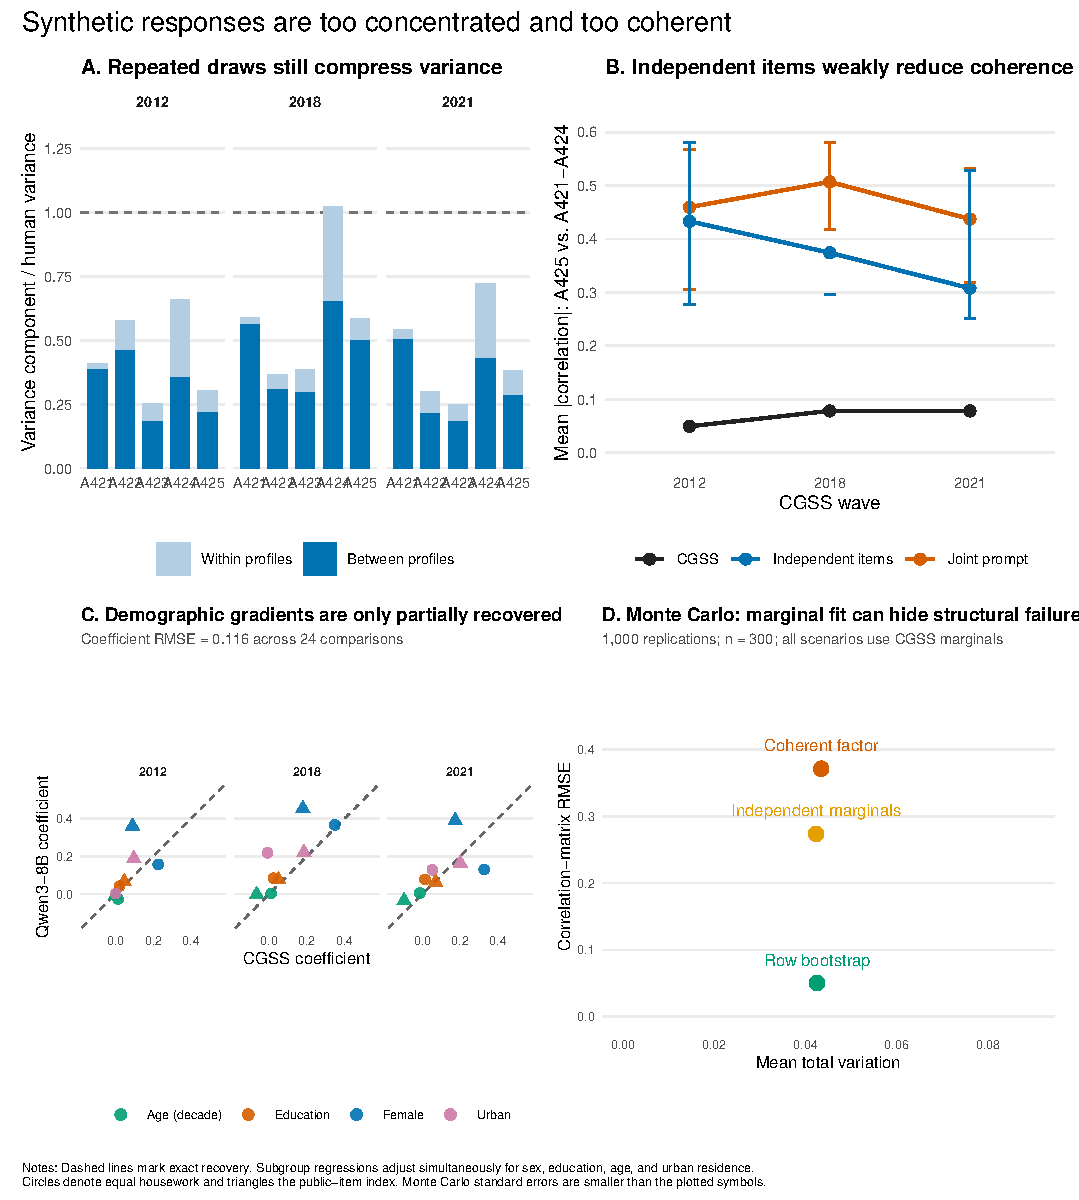
\includegraphics[width=\textwidth]{figures/structural_fidelity.pdf}
  \caption{Heterogeneity and relational fidelity. Panel C compares descriptive demographic
  coefficients for the public-item index and equal housework. Panel D reports the
  CGSS-calibrated Monte Carlo scenarios.}
  \label{fig:structural}
\end{figure*}

The model also imposes a joint ideology that the human data do not contain. In the weighted \CGSS
benchmark, the mean absolute correlation between A425 and A421--A424 is .049 in 2012 and .078 in
both 2018 and 2021. The corresponding Qwen3-8B values are .460, .507, and .437, absolute gaps of
.359--.429. Unweighted Pearson estimates are .051--.067, and unweighted polychoric estimates are
.069--.091, so neither weighting nor ordinal scaling explains the synthetic coherence.

Demographic gradients are partly, not fully, recovered. Across 24 coefficient comparisons for sex,
education, age, and urban residence, sign agreement is 83.3 percent and coefficient RMSE is .117.
Education gradients are often directionally similar, but the model overstates several sex
differences and misses some item-specific urban and household patterns. A model can therefore
produce broadly recognizable demographic sorting while still misrepresenting its magnitude and
domain specificity.

Independent presentation yields a smaller point estimate of excess coherence, but not a decisive
mechanism test. The mean joint-minus-independent contrast is .096, with a profile-bootstrap
95 percent interval of $[-.043,.156]$. Independent-item mean absolute correlations remain .433,
.374, and .308 across the three waves---still far above the weighted human values---while A422 and A424
become constant or nearly constant in several wave-item cells. The direction is compatible with
context-induced consistency, but the interval includes zero, the independent condition has only one
draw per profile-item, and the manipulation introduces a new heterogeneity failure. The defensible
conclusion is therefore narrower: the recorded presentation procedures differ, but the experiment
does not identify a unique internal mechanism and neither presentation recovers the observed
population structure.

\begin{figure*}[!htbp]
  \centering
  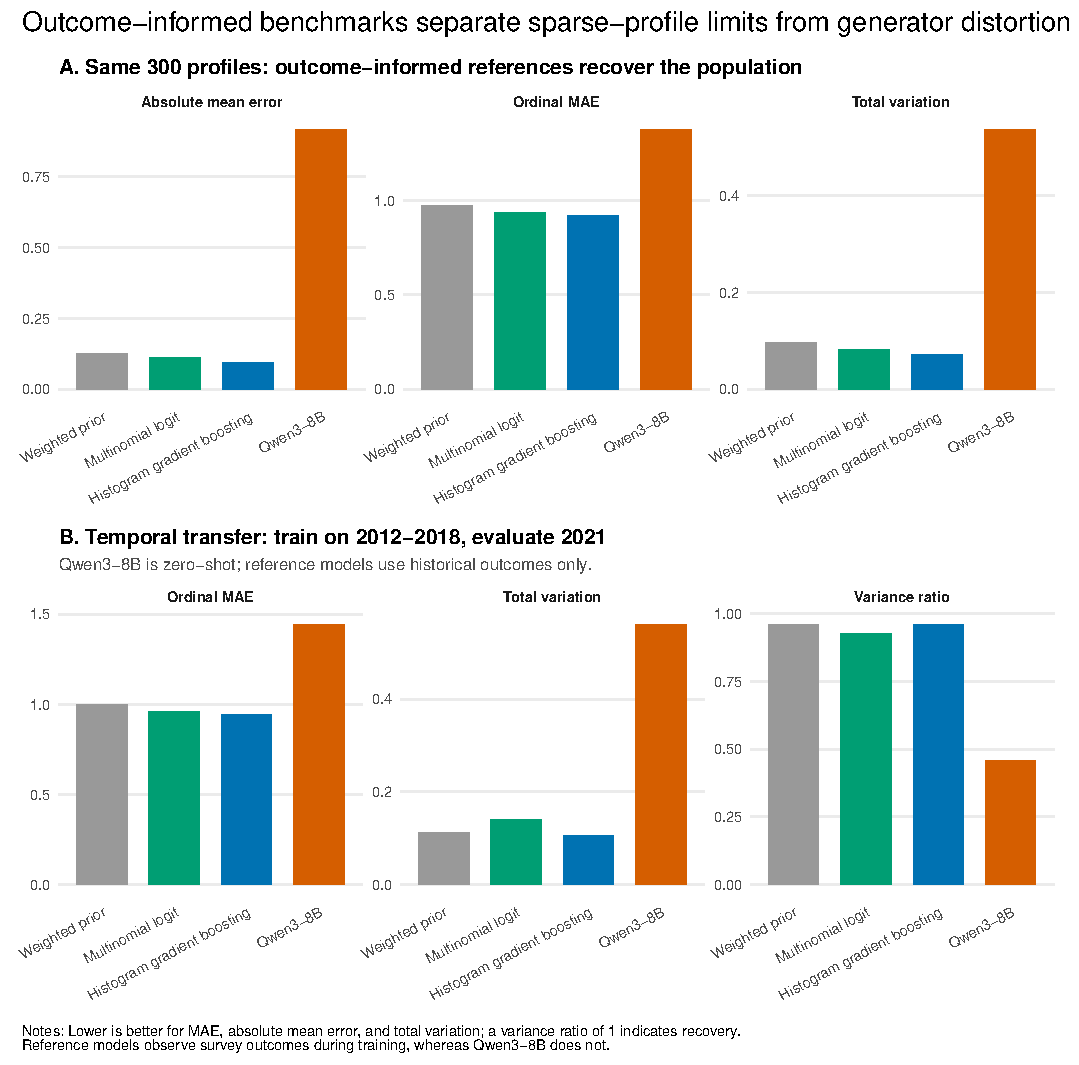
\includegraphics[width=\textwidth]{figures/benchmark_comparison.pdf}
  \caption{Matched-profile and temporal-transfer benchmarks. Lower values are better for ordinal
  MAE, absolute mean error, and total variation; one is the target for the variance ratio. The
  references are outcome-informed, whereas Qwen3-8B is zero-shot.}
  \label{fig:benchmark}
\end{figure*}

\ifdefined\SHOWCASE
  \clearpage
\fi
\subsection{Sparse profiles do not explain the full error}

Panel B of \cref{tab:core-results} and Panel A of \cref{fig:benchmark} address the main alternative
explanation. The supervised models remain imperfect at the individual level: \HGB's OMAE is .923
and multinomial logit's is .935. Demographic profiles therefore impose a genuine information
ceiling. But the reference models recover aggregate distributions far better than Qwen3-8B. \HGB's
total variation is .071 and variance ratio .987, compared with .538 and .466 for Qwen3-8B.

Even the weighted prior, which learns no mapping from profiles to answers, outperforms the LLM:
OMAE is .975, total variation .097, and variance ratio .992. This does not make the prior
information-free; it uses training-fold outcome frequencies. Its diagnostic value is that accurate
base rates alone recover more of this population than demographic conditioning through the
zero-shot LLM.

The joint-donor benchmark addresses the relational gap left by separate item classifiers. Despite
matching only on wave, sex, education group, and residence, it has OMAE .987, total variation .070,
variance ratio .973, correlation-matrix RMSE .085, and A425 mean absolute correlation .105. It is
not an optimal model, but it shows that preserving complete response vectors substantially restores
the human joint structure. The contrast is therefore not between an unattainable oracle and the LLM.

The paired individual comparison is also stable within the matched sample. Qwen3-8B's five-draw
profile-mean absolute ordinal error exceeds \HGB's by .456 points, with a profile-cluster bootstrap
interval of $[.407,.507]$. The gap is concentrated in employment protection and equal housework rather than
spread uniformly over the battery.

Temporal transfer provides a harder reference. On the exact 100-profile 2021 cohort used for the
LLM audit, training on 2012 and 2018 gives \HGB an OMAE of .945, total variation of .107, and variance
ratio of .959. Public opinion shifts, and survey-trained models pay a penalty for extrapolation.
Qwen3-8B on the same cohort has OMAE 1.44, total variation .561, and variance ratio .459.
Historical outcome information is not equivalent to zero-shot generation, but the comparison
shows that target-year exclusion alone does not produce the LLM's degree of distortion.

\section{Discussion}

\subsection{What the audit identifies---and what it does not}

The audit does not identify a pure architecture-level ``generator effect.'' The outcome-informed
references receive task-specific labels that the zero-shot LLM does not. What the audit establishes
is narrower: sparse demographic profiles are not a sufficient explanation for the recorded
distortion. Every model remains uncertain about individual gender attitudes, yet simple
outcome-informed references recover the marginal distribution, and a stratified joint donor
recovers much of the dependence structure. Sparse profiles therefore do not force a model to shift
item means, halve population variance, or transform a weakly related housework item into part of a
coherent ideology.

This distinction changes how synthetic respondents should be evaluated. Individual exact match,
aggregate calibration, heterogeneity, and relational structure are different targets. No single
accuracy score can certify them. The proposed procedure therefore begins with the intended
estimand:

\begin{itemize}[leftmargin=2em]
  \item For a population mean or category share, require marginal calibration and report uncertainty.
  \item For dispersion, polarization, or subgroup overlap, also require variance and tail recovery.
  \item For regressions, scales, latent classes, mediation, or networked attitudes, require joint and
  subgroup structure in addition to marginals.
  \item In every case, compare the LLM with a marginal prior and transparent task-specific learners
  so that failure is not attributed automatically to insufficient profile information.
  \item Calibrate tolerances against equally sized human samples rather than declaring success from
  an arbitrary numerical threshold.
\end{itemize}

The procedure is intentionally conservative. Passing does not prove that an LLM has learned the
human mechanism; it shows only that the generated data reproduce stated benchmark properties within
sampling-calibrated tolerances. Failing a required property is more informative: it rules out the
generated sample for estimands that depend on that property.

\subsection{Why synthetic coherence is substantively hazardous}

In the gender-attitude illustration, inconsistency is part of the phenomenon. Human respondents may
support public equality while assigning household obligations differently. The model replaces some
of this ambivalence with a single demographic narrative. The result is a sample that appears easier
to explain than the population it represents.

This error is particularly hazardous for computational social science. A researcher using the
synthetic data could conclude that the five items form a stronger scale, identify cleaner ideological
types, estimate steeper demographic gradients, or simulate more uniform attitude change. Each
conclusion would be supported by orderly synthetic patterns that are weak or absent in the survey.
The problem is not merely bias toward traditional or egalitarian answers. It is the production of a
different social structure.

The stakeholders extend beyond the analyst. Policy organizations that substitute synthetic
respondents for hard-to-reach populations may understate disagreement, erase minority combinations
of beliefs, or design interventions around a consensus that does not exist. The harm is
estimand-specific: mean distortion misstates prevalence, variance compression obscures pluralism,
and synthetic coherence can manufacture a scale or social type. Choosing \CGSS as the benchmark is
also a normative and empirical decision. It privileges a probability survey with explicit weights
over pretrained textual regularities, while acknowledging that the survey itself contains
nonresponse, item error, and wording effects.

The finding also qualifies cross-cultural claims about LLM public-opinion simulation. Prior work
documents uneven performance across countries and topics \parencite{qu2024performance}. The present
case adds a Chinese-language, open-weight model audit and shows why average country-level agreement
is insufficient. Cultural or linguistic representativeness must be evaluated in the relationships
among answers, not inferred from a plausible mean.

\subsection{Comparison with prior synthetic-respondent audits}

The design extends rather than contradicts existing evaluations. \textcite{argyle2023one} show that
demographic conditioning can recover nuanced response patterns in some settings.
\textcite{bisbee2024synthetic} demonstrate failures in means, variances, conditional relationships,
prompt sensitivity, and reproducibility. The present contribution adds two pieces. First, the
Monte Carlo study makes explicit that marginal validation is non-identifying for joint structure.
Second, the human-sampling envelope and outcome-informed reference ladder turn that insight into a
falsification procedure. The answer in this application is partial: sparse persona attributes
explain why no method predicts individuals perfectly, but they do not account for the recorded
Qwen3-8B population. The design still cannot determine whether the remaining gap comes from model
architecture, pretraining, prompt interpretation, or the absence of target-specific calibration.

This logic can travel beyond gender attitudes. Researchers evaluating synthetic respondents for
health beliefs, consumer preferences, political ideology, or experimental behavior can replace the
items and reference models while retaining the four-stage audit. The required relational diagnostic
should follow the intended analysis: correlations for scale construction, treatment-effect
heterogeneity for experiments, transition matrices for panels, or network statistics for social
interaction.

\section{Limitations and Required Next Tests}

Seven limitations bound the evidence.

First, the empirical audit concerns one open-weight model and one parameter scale. Qwen3-8B is useful
for reproducibility and local data protection, but a single model cannot support a claim about all
LLMs. Cross-family and within-family scaling comparisons are the highest-priority extension.

Second, five draws provide an empirical predictive distribution, but they remain a coarse
approximation to the model's option probabilities. They identify within-profile stochastic
variation more credibly than a single draw, yet cannot support fine-grained entropy or calibration
analysis. Direct candidate-token probabilities would provide a stronger probabilistic comparison.

Third, independent presentation changes the amount of questionnaire context by design and was
generated only once per profile-item, whereas the joint condition has five repeats. The resulting
contrast identifies neither a unique internal mechanism nor the full decoding uncertainty under
independent presentation. Moreover, an item with nearly constant independent responses has no
well-defined Pearson correlation; reduced correlation cannot then be interpreted as repaired
relational fidelity without also checking heterogeneity.

Fourth, the original prompt ablation still changes both social-desirability wording and response
format. It demonstrates sensitivity but does not identify which component causes it. A future
factorial design should vary instruction, verbal labels, presentation mode, temperature, and seed
separately.

Fifth, the survey battery has a measurement limitation. A425 is one positively worded item, whereas
A421--A424 are traditional statements that are reverse-coded. Human weak covariance may reflect
domain separation, wording, or both. Replication with multi-item public and household measures is
needed before treating the observed structure as a general latent model of gender ideology.

Sixth, the sampling envelope treats the full weighted \CGSS sample as the benchmark and reproduces
the profile-selection stage rather than the original survey's complete multistage design. It
calibrates finite-profile error but does not propagate all PSU, stratification, nonresponse, and
weight-estimation uncertainty.

Seventh, the contents of Qwen3-8B's pretraining corpus are not fully observable. The model may have
encountered the item wording, discussions of \CGSS, or related normative language. Prompt
paraphrases and temporal comparisons diagnose sensitivity, but they cannot identify contamination
or memorization.

These limitations affect the breadth and mechanism of the claim, not the observed failure of the
recorded Qwen3-8B procedure. The synthetic sample produced here does not recover the population
properties required for scale, regression, or latent-structure analysis.

\section{Conclusion}

Synthetic respondents should be audited as populations. A plausible answer from a plausible persona
does not establish correct base rates, disagreement, covariance, or subgroup structure. The
population-fidelity audit turns that principle into a staged diagnostic tied to the intended
estimand.

In a CGSS-calibrated simulation, generators with nearly indistinguishable marginal fit produce
radically different joint distributions. In the empirical illustration, Qwen3-8B shifts several
gender-attitude means, compresses variance, and imposes much stronger ideological coherence than
appears among human respondents. Its errors lie outside the reference envelopes produced by
equally sized human samples in every audited wave-property cell. Outcome-informed references
confirm that demographic profiles contain limited individual information, but they also show that
this limitation alone does not account for the LLM's specific population distortion.

The practical recommendation is direct: do not validate synthetic respondents with means alone, do
not interpret low individual accuracy without an outcome-informed predictive benchmark, and do not use
synthetic data for relational estimands until the relevant joint structure has been recovered.

\section*{Preregistration Statement}

The study was not registered in a public repository before analysis. After the initial audit, but
before completing the follow-up model calls, the repeated-draw estimand, profile-level bootstrap,
independent-item manipulation, and sign of the joint-minus-independent correlation contrast were
fixed in the dated analysis log. The follow-up is therefore specification-before-completion rather
than a formal preregistration.

\section*{Code, Materials, and Data Availability}

\begin{sloppypar}
The code-only replication archive accompanying this writing sample contains the prompt templates,
model-call runner, survey-trained benchmark code, Monte Carlo code, and aggregate results supporting
the displayed analyses. Respondent-level \CGSS data, derived persona files, matched human responses,
and profile-level model logs are not part of the public release because access is governed by the
data provider and the derived records remain linked to sampled profiles. Qualified researchers can
obtain the source waves from the National Survey Research Center at Renmin University of China,
rebuild the derived files locally, and regenerate the local-model calls. Before journal submission,
the code-only review archive should be deposited in a blinded repository and assigned a permanent
DOI upon acceptance.
\end{sloppypar}

\section*{Ethics and Consent Statement}

The study is a secondary analysis of deidentified survey data and generated model outputs. No new
human participants were recruited or contacted.

\section*{Declaration of Conflicting Interests}

The author declared no potential conflicts of interest with respect to the research, authorship,
and/or publication of this article.

\section*{Funding Statement}

The author received no financial support for the research, authorship, and/or publication of this
article.

\section*{Declaration of Generative AI Use}

During preparation of this manuscript, the author used OpenAI Codex to assist with code review,
figure production, manuscript restructuring, and language editing. The author reviewed the
analyses, verified reported results against local outputs, edited the generated text, and takes full
responsibility for the content.

\printbibliography[title={References}]

\end{document}
